\documentclass[10pt]{beamer}
\usepackage{amsmath,amssymb,longtable,hhline}
\usepackage{mathrsfs}
\usepackage{xcolor}
\usepackage{listings}
\usepackage{hyperref}

\definecolor{mygreen}{rgb}{0,0.6,0}
\definecolor{mygray}{rgb}{0.5,0.5,0.5}
\definecolor{mymauve}{rgb}{0.58,0,0.82}

\hypersetup{
    bookmarks=true,         % show bookmarks bar?
    unicode=true,           % non-Latin characters in Acrobat’s bookmarks
    pdftoolbar=false,        % show Acrobat’s toolbar?
    pdfmenubar=false,        % show Acrobat’s menu?
    pdffitwindow=false,     % window fit to page when opened
    pdfstartview={FitH},    % fits the width of the page to the window
    pdftitle={Компьютерная алгебра в задачах оптимизации},    % title
    pdfauthor={Evgeny Cherkashin, Seseg Badmatsyrenova},     % author
    pdfsubject={symbolic computations},   % subject of the document
    pdfnewwindow=true,      % links in new PDF window
    colorlinks=true,       % false: boxed links; true: colored links
    linkcolor=red,          % color of internal links (change box color with linkbordercolor)
    citecolor=green,        % color of links to bibliography
    filecolor=magenta,      % color of file links
    urlcolor=blue           % color of external links
}

\lstset{language=Python,
  basicstyle=\footnotesize\ttfamily,        % the size of the fonts that are used for the code
  breakatwhitespace=false,         % sets if automatic breaks should only happen at whitespace
  breaklines=true,                 % sets automatic line breaking
  captionpos=b,                    % sets the caption-position to bottom
  commentstyle=\color{mygreen},    % comment style
  escapeinside={\%*}{*)},          % if you want to add LaTeX within your code
  extendedchars=true,              % lets you use non-ASCII characters; for 8-bits encodings only, does not work with UTF-8
%  frame=single,                    % adds a frame around the code
  keepspaces=true,                 % keeps spaces in text, useful for keeping indentation of code (possibly needs columns=flexible)
  keywordstyle=\color{blue},       % keyword style
%  numbers=left,                    % where to put the line-numbers; possible values are (none, left, right)
  numbersep=5pt,                   % how far the line-numbers are from the code
  numberstyle=\tiny\color{mygray}, % the style that is used for the line-numbers
  rulecolor=\color{black},         % if not set, the frame-color may be changed on line-breaks within not-black text (e.g. comments (green here))
  showspaces=false,                % show spaces everywhere adding particular underscores; it overrides 'showstringspaces'
  showstringspaces=false,          % underline spaces within strings only
  showtabs=false,                  % show tabs within strings adding particular underscores
  stepnumber=2,                    % the step between two line-numbers. If it's 1, each line will be numbered
  stringstyle=\color{mymauve},     % string literal style
  tabsize=2,                       % sets default tabsize to 2 spaces
%  title=\lstname                   % show the filename of files included with \lstinputlisting; also try caption instead of
}

\usetheme{Warsaw}
\usecolortheme{crane}
\beamertemplatenavigationsymbolsempty

\usepackage{iftex,ifxetex}
\ifPDFTeX
  \usepackage[utf8]{inputenc}
  \usepackage[T1]{fontenc}
  \usepackage[russian]{babel}
  \usepackage{lmodern}
  \usefonttheme{serif}
\else
  \ifluatex
    \usepackage{unicode-math}
    \defaultfontfeatures{Ligatures=TeX,Numbers=OldStyle}
    \setmathfont{Latin Modern Math}
    \setsansfont{Linux Biolinum O}
    \usefonttheme{professionalfonts}
    \setmathfont[
        Ligatures=TeX,
        Scale=MatchLowercase,
        math-style=upright,
        vargreek-shape=unicode
        ]{euler.otf}
  \fi
\fi

%\useoutertheme{split}
%\useinnertheme{rounded}
\setbeamertemplate{background canvas}[vertical shading][bottom=white!80!cyan!20,top=cyan!10]
%\setbeamertemplate{sidebar canvas left}[horizontal shading][left=white!40!black,right=black]

\graphicspath{{pics/}}


% --------------------------

\begin{document}
\title[КОМПЬЮТЕРНАЯ АЛГЕБРА В ЗАДАЧАХ ОПТИМИЗАЦИИ]{ПРИМЕНЕНИЕ КОМПЬЮТЕРНОЙ АЛГЕБРЫ\\
В РЕАЛИЗАЦИИ АЛГОРИТМОВ УЛУЧШЕНИЯ}
\author{Черкашин Е.А., Бадмацыренова С.Б.}
\institute[ИДСТУ СО РАН, ИРНИТУ, ИМЭИ ИГУ]{\normalsize  ИДСТУ СО РАН, ИРНИТУ, ИМЭИ ИГУ}
\date[2015]{{}\\[1.5cm]
<<Винеровские чтения --- 2015>>\\
16 -- 18 апреля 2015 г.,
Иркутск
}
%\date{\today}
\maketitle

% ----------------------------------------------------------------
\begin{frame}{\textbf{Вектор-функция} }
%\begin{block}{}
  \begin{columns}[t]
    \begin{column}{0.65\textwidth}\footnotesize
      \def\xyz{$x_1,x_2,x_3,\;x_4,x_5,x_6$} \def\yaw{$x_7,x_8$} \def\pitch{$x_9,x_{10}$}
      \def\roll{$\!\!\!\!\!\!x_{11},x_{12}$} \def\lift{$x_{13}$} \def\down{$\!\!x_{14}$}
      \def\thrust{$u_1$} \def\rudder{$u_5$} \def\drag{$x_{15}$}
      \def\flaps{$u_2$} \def\aeleron{$u_3$} \def\engine{}
      \def\elevator{$u_4$} \def\svgwidth{\columnwidth}
      \input{pics/Cessna-Plane.pdf_tex}
    \end{column}
    \begin{column}{0.35\textwidth}
      \begin{block}{Состояние, управление}%
        \vspace{-1.5em}
        \begin{align*}
          &\vec{x}=\mathbf{x}=\langle x_1,x_2,\ldots,x_n\rangle,\\
          &n=15,\\
          &\vec{u}=\mathbf{u}=\langle u_1,u_2,\ldots,u_m\rangle,\\
          &m=5,\\
          &\vec{f}=\mathbf{f}.
        \end{align*}
      \end{block}
    \end{column}
  \end{columns}
%\end{block}
\begin{block}{Уравнение движения (Задача Коши)}
  \begin{align*}
&\dot{\mathbf{x}}=\frac{\mathbf{x}(t)}{dt}=\mathbf{f}(t,\mathbf{x}(t),\mathbf{u}(t)),\quad t \in T=[t_0,t_1], \\
&\mathbf{x}(t_0)=\mathbf{x}_0,\quad \mathbf{x}(t)\in \mathbb{R}^n,\; \mathbf{u}(t) \in \mathbb{R}^m,\quad t\in T, \\
&I(\mathbf{x},\mathbf{u})=\int\limits_{t_0}^{t_1}f^0(t,\mathbf{x}(t),\mathbf{u}(t))dt \to \min.
  \end{align*}
\end{block}
\end{frame}
\begin{frame}{\textbf{Постановка задачи} }
\begin{block}{Дискретный вариант уравнения движения (Задача Коши)}
  \begin{align}
&\mathbf{x}(t+1)=\mathbf{f}(t,\mathbf{x}(t),\mathbf{u}(t)),\quad t \in T=\{t_0,t_0+1,...,t_1\},
	\label{eq100} \\
&\mathbf{x}(t_0)=\mathbf{x}_0,\quad \mathbf{x}(t)\in \mathbb{R}^n,\; \mathbf{u}(t) \in \mathbb{R}^m,\quad t\in T,\label{eq100a} \\
&I(\mathbf{x},\mathbf{u})=F(\mathbf{x}(t_1))+ \sum_{t_0}^{t_1-1}f^0(t,\mathbf{x}(t),\mathbf{u}(t)) \to \min.
  \label{eq103}
  \end{align}
\end{block}
\begin{block}{Задача улучшения}
  Пусть заданы управление $\mathbf{u}^I(t)$ и соответствующее состояние $\mathbf{x}^I(t)$. Требуется найти $\mathbf{x}^{I\!I}(t),$ $\mathbf{u}^{I\!I}(t)$ такие, что
\[
I(\mathbf{x}^{I\!I},\mathbf{u}^{I\!I}) < I(\mathbf{x}^I,\mathbf{u}^I).
\]
 \end{block}
\end{frame}
% ---------------------------------------------------------
\def\H{\mathbf{H}}
\def\x{\mathbf{x}}
\def\u{\mathbf{u}}
\def\f{\mathbf{f}}
\def\F{\mathbf{F}}
\def\bpsi{\psi\hspace{-.68em}\psi\hspace{-.68em}\psi}
% ----------------------------------------------------------------
\begin{frame}[shrink]{\textbf{Алгоритм первого порядка} }
%\begin{block}{}
\begin{enumerate}
 \item[1.] Задается начальное управление $\mathbf{u}^I(t)$, из уравнения \eqref{eq100} и условий \eqref{eq100a} определяется $\mathbf{x}^I(t)$. Вычисляется $I(\mathbf{x}^I,\mathbf{u}^I).$
 \item[2.] Из системы $\mathbf{\psi}(t)=\mathbf{H}_\mathbf{x},\;\bpsi(t_1)=-\F_\x,$ находим $\bpsi(t),$\\ где $\bpsi(t)$ --- $n$-вектор, $\H_\u(t,\x,\bpsi(t+1),\u)=\bpsi^{T}(t+1)\times\f(t,\x,\u)-f^{0}(t,\x,\u),$ производные функции $H$ по $\u$ ($\H_\u$) находятся в точке $\left(t,\x^{I}(t),\bpsi \left(t+1 \right),\u^{I}(t)\right)$. Задается параметр $\alpha$.
 \item[3.] Из системы $\x(t+1)=\f(t,\x(t),\u^{I\!I}(t)), \x(t_0)=\x_0,$ где $\u^{I\!I}(t)=\u^{I}(t)+\alpha \H_\u,$ вычисляется $\x^{I\!I}(t).$
 \item[4.] Новое управление и значение параметра $\alpha$ подсчитываются из решения задачи одномерной минимизации для функционала $I(\x^{I\!I},\u^{I\!I})\to \min\limits_{\alpha}.$
 \item[5.] Если $I\left(\x^{I\!I},\u^{I\!I}\right)\geq I\left(\x^{I},\u^{I}\right)$ (улучшение не произошло), то уменьшаем $\alpha$ и переходим к следующей итерации, начиная с пункта~3.
 \item[6.] Иначе, если $I\left(\x^{I\!I},\u^{I\!I}\right) - I\left(\x^{I},\u^{I}\right)>\epsilon$, то переходим к следующей итерации, начиная с пункта~2. Значение $\epsilon$ --- параметр точности.
\end{enumerate}
%\end{block}
\end{frame}
% ----------------------------------------------------------------

\begin{frame}[fragile]{Задание модели}
\begin{lstlisting}
class LinModel1(Model):
    def __init__(self):
        X0=(1.0,)
        self.h = Ht
        self.num = int((1.0-0.0) / self.h)
        self.T = linspace(start=0.0, stop=1.0, num=self.num)
        self.t = arange(len(self.T))
        Model.__init__(self, X0=X0, U0=self.start_control())

    def start_control(self):
        U = [(0.0,) for t in self.t[:-1]]
        return array(U)

    def F(self, x):
        return 0.0

    def f(self, t, x, u):
        x0=x[0]; u0=u[0]
        return (x0+self.h*u0,)

    def f0(self, t, x, u):
        x0=x[0]; u0=u[0]
        return self.h * (x0*x0+u0*u0)
\end{lstlisting}
\end{frame}
\begin{frame}[fragile]
  \frametitle{Реализация алгоритма улучшения}
\begin{lstlisting}
class Process(VFCalc):
    def __init__(self, model, alpha=1.0):
        VFCalc.__init__(self, model.N, model.M)
        t,x,u=self.v.t,self.v.x,self.v.u
        self.model=model; self.alpha=alpha
        self.v.f=model.f(t, x, u)
        self.v.f0=model.f0(t, x, u)
        self.v.F=model.F(x)

    def trajectory(self, U):
        x0=self.model.X0; X = [x0]
        for t, u in enumerate(U): # (0, u0), (1, u1)
            xn=self.model.f(t, X[t], u); X.append(xn)
        return array(X)

    def I(self, X, U):
        def _a(acc, t):
            return acc + self.model.f0(t, X[t], U[t])
        return reduce(_a, range(len(X)-1), self.model.F(X[-1]))

    def optimize(self, t, eps=0.001, iters=1000):
        Up=self.model.U0
        Xp=self.trajectory(Up)
        Ip=self.I(Xp,Up); it = 1
\end{lstlisting}
\end{frame}
\begin{frame}[fragile]
  \frametitle{Реализация алгоритма улучшения (\texttt{optimize})}
\begin{lstlisting}
        while True:
            beta = self.beta
            Psi=self.Psi(t, Xp, Up, self.alpha)
            _H_u=self.H((self.v.u,), t[:-1], Xp[:-1], Up, Psi)
            while True:
                _dU=_H_u*alpha
                Un = Up + _dU
                Xn = self.trajectory(Un)
                In = self.I(Xn, Un)
                dI = Ip-In
                if abs(dI)<eps:
                    return In, Xn, Un, it, "Opt"
                if iters<=0:
                    return In, Xn, Un, it, "Nonoptimal"
                iters-=1; it+=1
                if In>=Ip:
                    alpha/=2
                    continue
                else:
                    Xp, Up, Ip = Xn, Un, In
                    break
\end{lstlisting}
\end{frame}
\begin{frame}[fragile]
  \frametitle{Реализация алгоритма улучшения (\texttt{psi, H})}
\begin{lstlisting}
    def Psi(self, t, X, U, alpha):
        v=self.v
        psie = -self.fun(v.F,(v.x,), t[-1], X[-1], U[-1])
        psi=[psie]; X=X[:-1]; t=t[:-1]
        _f0_x=self.fun(v.f0, (v.x,), t, X, U) # Vector context
        _f_x =self.fun(v.f, (v.x,), t, X, U)  # Vector context
        j=len(t)-1; p=psie
        while j>=1:
            i=t[j]; pp=p
            pn = dot(pp, _f_x[i]) - alpha*_f0_x[i]
            psi.append(pn); p=pn; j-=1
        psi=array(psi)
        return psi[::-1]

    def H(self, vars, T, X, U, Psi, alpha = 1.0):
        f=self.fun(self.v.f, vars, T, X, U)
        f0=-self.fun(self.v.f0, vars, T, X, U)
        H = alpha * f0
        for psi,_H,_f,i in zip(Psi, H, f, range(len(H))):
            _H += dot(psi,_f); H[i]=_H
        return H
\end{lstlisting}
\end{frame}
\begin{frame}[fragile]
  \frametitle{Реализация алгоритма улучшения (\texttt{fun})}
\begin{lstlisting}
    def fun(self, f, vars, T, X, U):
        code,df=self.code(f, *vars)
        X=numpy.atleast_1d(X)
        U=numpy.atleast_1d(U)
        if X.ndim>1:
            Xs=[X[:,i:i+1] for i in range(X.shape[1])]
            Us=[U[:,i:i+1] for i in range(U.shape[1])]
            m,args=True,(T,)+tuple(Xs+Us)
        else:
            m,args=False,(T,)+tuple(X)+tuple(U)
        rc=code(*args)
        rct=type(rc)
        rc=numpy.atleast_1d(rc)
        if type(T)==numpy.ndarray:
            try:
                if rct in [TupleType,ListType]:
                    rc=rc.reshape(rc.shape[:-1])
                    rc=rc.T
                    return rc
            except ValueError: pass
            if T.shape[0]!=rc.shape[0]:
                nrc=numpy.zeros((len(T),)+rc.shape,dtype=float)
                nrc[:]=rc; rc=nrc
        return rc
\end{lstlisting}
\end{frame}
\begin{frame}[fragile]
  \frametitle{Выполнение теста}
\begin{columns}
\begin{column}{0.43\columnwidth}
\vspace{-3em}
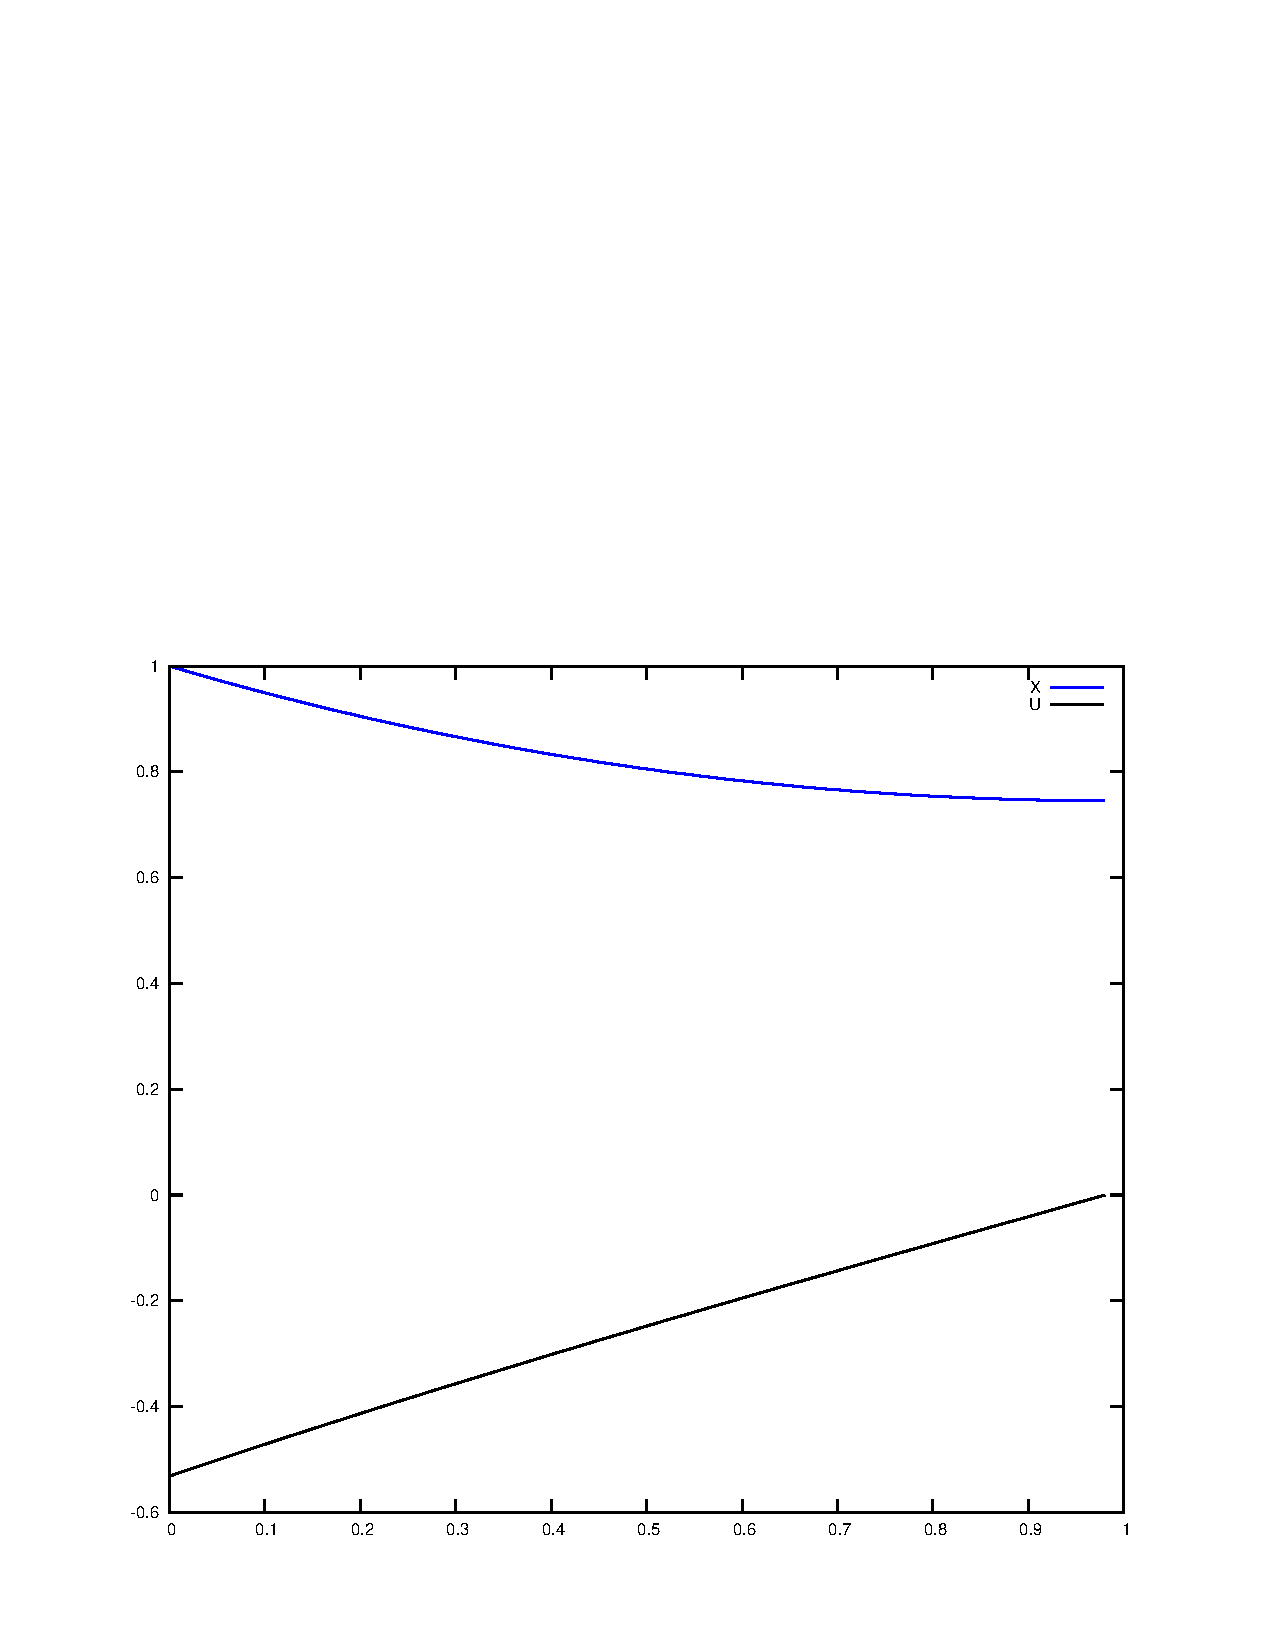
\includegraphics[width=1.2\textwidth]{1dplot}
\vspace{1em}
\texttt{I: 0.77666 iters: 47}
\end{column}
\begin{column}{0.57\columnwidth}
\begin{lstlisting}
def test_with_plot():
    m = LinModel1()
    p1=Process(m, beta=1.0)
    iters=2000
    eps=0.001
    print ("First-order process:")
    print ("-"*20)
    r1=I1, X1, U1, it1, _1 =
        p1.optimize(m.t, eps=eps,
            iters=iters)
    print (I1, "iters:", it1)
    gnuplot("test_with_plt", r1)
\end{lstlisting}
\end{column}
\end{columns}
\end{frame}
\begin{frame}[fragile,plain]
  \frametitle{Дифференцирование вектор-функций}
  \begin{columns}[c]
    \begin{column}{0.45\columnwidth}
      \begin{block}{}
        \begin{align*}
          &\f=\langle f^1,f^2,\ldots,f^n\rangle\; (1\times n),\\
          &\x=\langle x_1,x_2,\ldots,x_n\rangle\; (1\times n),\\
          &\u=\langle u_1,u_2,\ldots,u_m\rangle\; (1\times m).\\
        \end{align*}
      \end{block}
    \end{column}
    \begin{column}{0.05\columnwidth}
      $$\implies$$
    \end{column}
    \begin{column}{0.5\columnwidth}
      \begin{block}{}
\[\f_x =
 \begin{pmatrix}
  f^1_1 & f^2_1 & \cdots & f^n_1 \\
  f^1_2 & f^2_2 & \cdots & f^n_2 \\
  \vdots  & \vdots  & \ddots & \vdots  \\
  f^1_n & f^2_n & \cdots & f^n_n
 \end{pmatrix}\; (n\times n)\]

Производная $\f_u$ имеет размерность $(m\times n)$,\goodbreak $\f_{x,x}$ --- $(n\times n\times n).$
      \end{block}
    \end{column}
  \end{columns}
  \begin{block}{Пример вычисления производной вектор-функции}
    \begin{columns}[t]
      \begin{column}{0.55\columnwidth}
\vspace{-1em}
\begin{lstlisting}
  d=VFCalc(2,2)
  x1,x2=Symbol('x1'),Symbol('x2')
  u1,u2=Symbol('u1'),Symbol('u2')
  y1=x1**2*u1+x2*u2**2
  y2=x1**2*x2**2*u1**2*u2**2
  res=(d.diff([y1,y2],
      [x1,x2], [u1,u2]))
  pprint (res)
  return
\end{lstlisting}
      \end{column}
      \begin{column}{0.45\columnwidth}
\begin{lstlisting}
(((2*x1, 0), (0, 2*u2)),
 ((4*u1*u2**2*x1*x2**2,
   4*u1**2*u2*x1*x2**2),
  (4*u1*u2**2*x1**2*x2,
   4*u1**2*u2*x1**2*x2)))
\end{lstlisting}
      \end{column}
    \end{columns}
  \end{block}
\end{frame}
\begin{frame}[fragile]
  \frametitle{Компьютерная алгебра: дифференцирование вектор-функций}
\begin{lstlisting}
class VFCalc(object):
    def __init__(self, N,M):
        self.N=N; self.M=M; self.v=Helper()
        self.v.x=[Symbol('x'+str(i+1)) for i in range(self.N)]
        self.v.u=[Symbol('u'+str(i+1)) for i in range(self.M)]
        self.v.t=Symbol('t')

    def diff1(self, f, var):
        if type(f) in [TupleType,ListType]:
            df=tuple([self.diff1(fi, var) for fi in f])
        else:
            df=tuple([diff(f, vi) for vi in var])
        if len(df)==1: df=df[0]
        return df

    def diff(self, f, *vars):
        cf=f
        for v in vars:
            cf=self.diff1(cf, v)
        return cf
\end{lstlisting}
\end{frame}
\begin{frame}[fragile]{Компьютерная алгебра: дополнительные функции}
\begin{lstlisting}
class VFCalc(object):
    # . . . . . . . .
    def subs(self, f, s):
        if type(f) not in [TupleType,ListType]:
            return f.subs(s) # common subs
        return tuple([self.subs(fi,s) for fi in f])#local subs

    def lambdify(self, f):
        l=[self.v.t]
        l.extend(self.v.x)
        l.extend(self.v.u)
        fl=lambdify(l, f, "numpy")
        return fl

    def code(self, f, *vars):
        df=self.diff(f, *vars)
        c=self.lambdify(df)
        return c,df
\end{lstlisting}
\end{frame}
% \begin{frame}
%   \frametitle{Пример вычисления производных вектор-функций}

% \end{frame}

%------------ Conclusion ----------------------------------------
\begin{frame}{Заключение}
  \begin{block}{Результаты}
    \begin{itemize}
    \item Разработана первая версия библиотеки дифференцирования
      вектор-функций, поддерживающей библиотеки \texttt{numpy}
      и \texttt{scipy};
    \item Использование библиотеки продемонстрировано на примере;
    \item Осуществляется реализация метода второго порядка.
    \end{itemize}
    Использование библиотеки позволяет повысить и точность и
    производительность вычислений.
  \end{block}
\begin{block}{Задачи на будущее}
  \begin{itemize}
  \item На основе методов \texttt{diff}, \texttt{lambdify} и \texttt{fun} реализовать генераторы кода разных вариантов $\f$, $\f^0$, $\F$.
  \item Разработать эффективные процедуры для вычисления $\bpsi$, $\H_\u$ и $\x$.
  \item Разработать методику представления схемы алгоритма улучшения и странслировать ее реализацию в компилируемый язык (C, C++, Fortran и т.~п.).
  \end{itemize}
\end{block}
\end{frame}

\begin{frame}{}
\vfill\vfill\vfill
\vfill
\begin{center}
  {\Huge\textbf{Спасибо за внимание!}}
\vspace{4em}
  \begin{block}{}
    Постоянный адрес презентации\,: \url{https://github.com/eugeneai/paropt/raw/exp/talk-2015-04-17-wiener.pdf}\\[1em]

  Презентация сверстана в пакете \LaTeX\ Beamer.
  \end{block}
\end{center}
\end{frame}
% ----------------------------------------------------------------

\end{document}
%

%%% Local Variables:
%%% mode: latex
%%% TeX-master: t
%%% End:
